\phantomsection
\addcontentsline{toc}{chapter}{Appendices}

% The \appendix command resets the chapter counter, and changes the chapter numbering scheme to capital letters.
%\chapter{Appendices}
\appendix

% \chapter{An Appendix About Stuff}
% \label{appendixlabel1}

% \chapter{Another Appendix About Things}
% \label{appendixlabel2}

\chapter{Colophon}
\label{appendixlabel3}

This document has been written with \LaTeX, within a mix of TeXworks (locally) and Overleaf (when online), based on a template created by Ian Kirker\footnote{\url{https://github.com/UCL/ucl-latex-thesis-templates}}.

In addition to the packages used in the template, additional use was made of package `libertine'\footnote{\url{https://ctan.org/pkg/libertine}}, which loads the Linux Libertine and Linux Biolinum font families which are free and open fonts\footnote{\url{http://libertine-fonts.org/}}. %and `microtype' which !!!!!!!!!!!!!!!, also lineno \\
%List other added packages
Zotero and Bib\TeX were used for reference management.

During writing git was used as a version control software, pushing to GitHub. See this thesis as a GitHub repo\footnote{\url{https://github.com/da5nsy/Thesis}}. %at the point of submission and as an updated repo (who knows if I will find typos later!)

% PTB



%\textit{This is a description of the tools you used to make your thesis. It helps people make future documents, reminds you, and looks good.}
%
%\textit{(example)} This document was set in the Times Roman typeface using \LaTeX\ and Bib\TeX , composed with a text editor. 
 % description of document, e.g. type faces, TeX used, TeXmaker, packages and things used for figures. Like a computational details section.
% e.g. http://tex.stackexchange.com/questions/63468/what-is-best-way-to-mention-that-a-document-has-been-typeset-with-tex#63503

% Side note:
%http://tex.stackexchange.com/questions/1319/showcase-of-beautiful-typography-done-in-tex-friends

\chapter{Ethics Application 9357/001}
\label{app:ethics3}
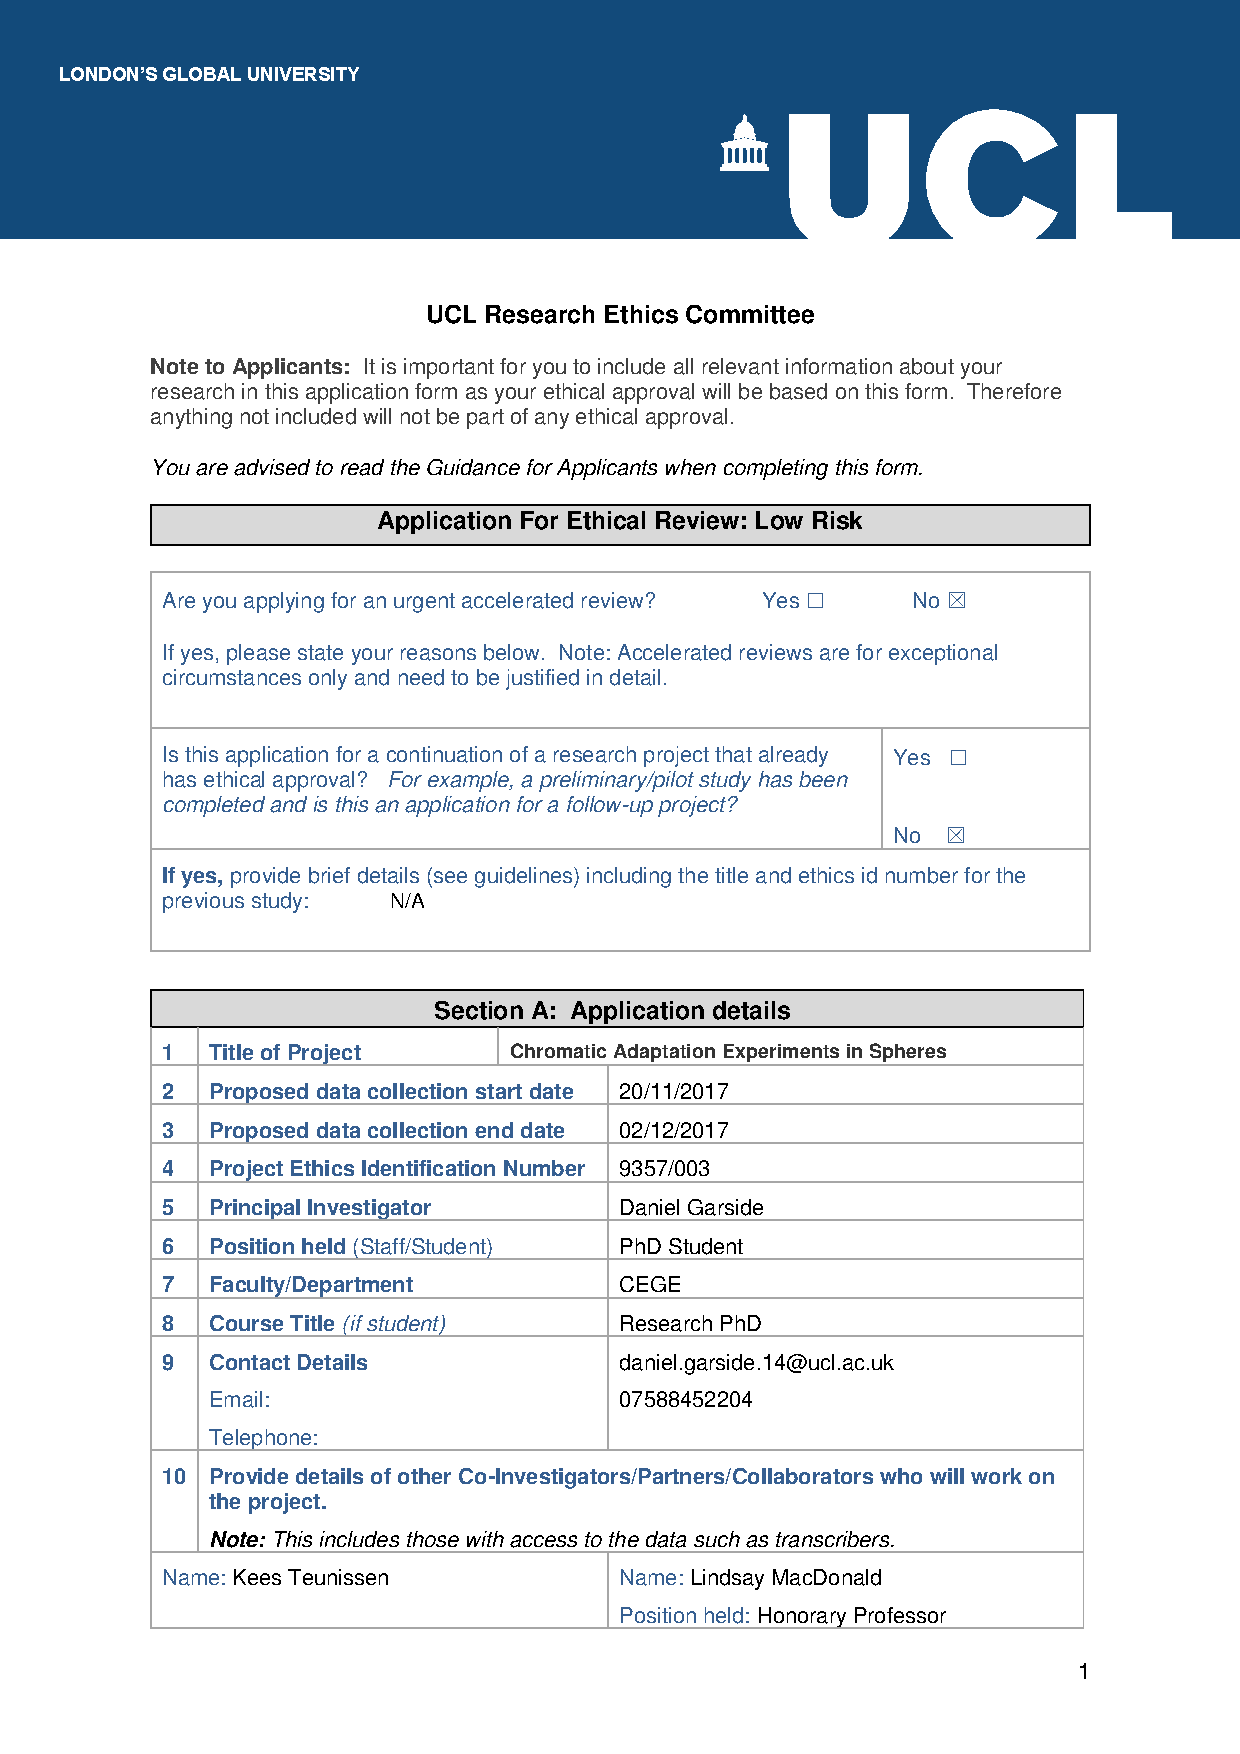
\includepdf[pages=1-22,scale=0.8]{ethics3.pdf}
\label{app:ethics1}
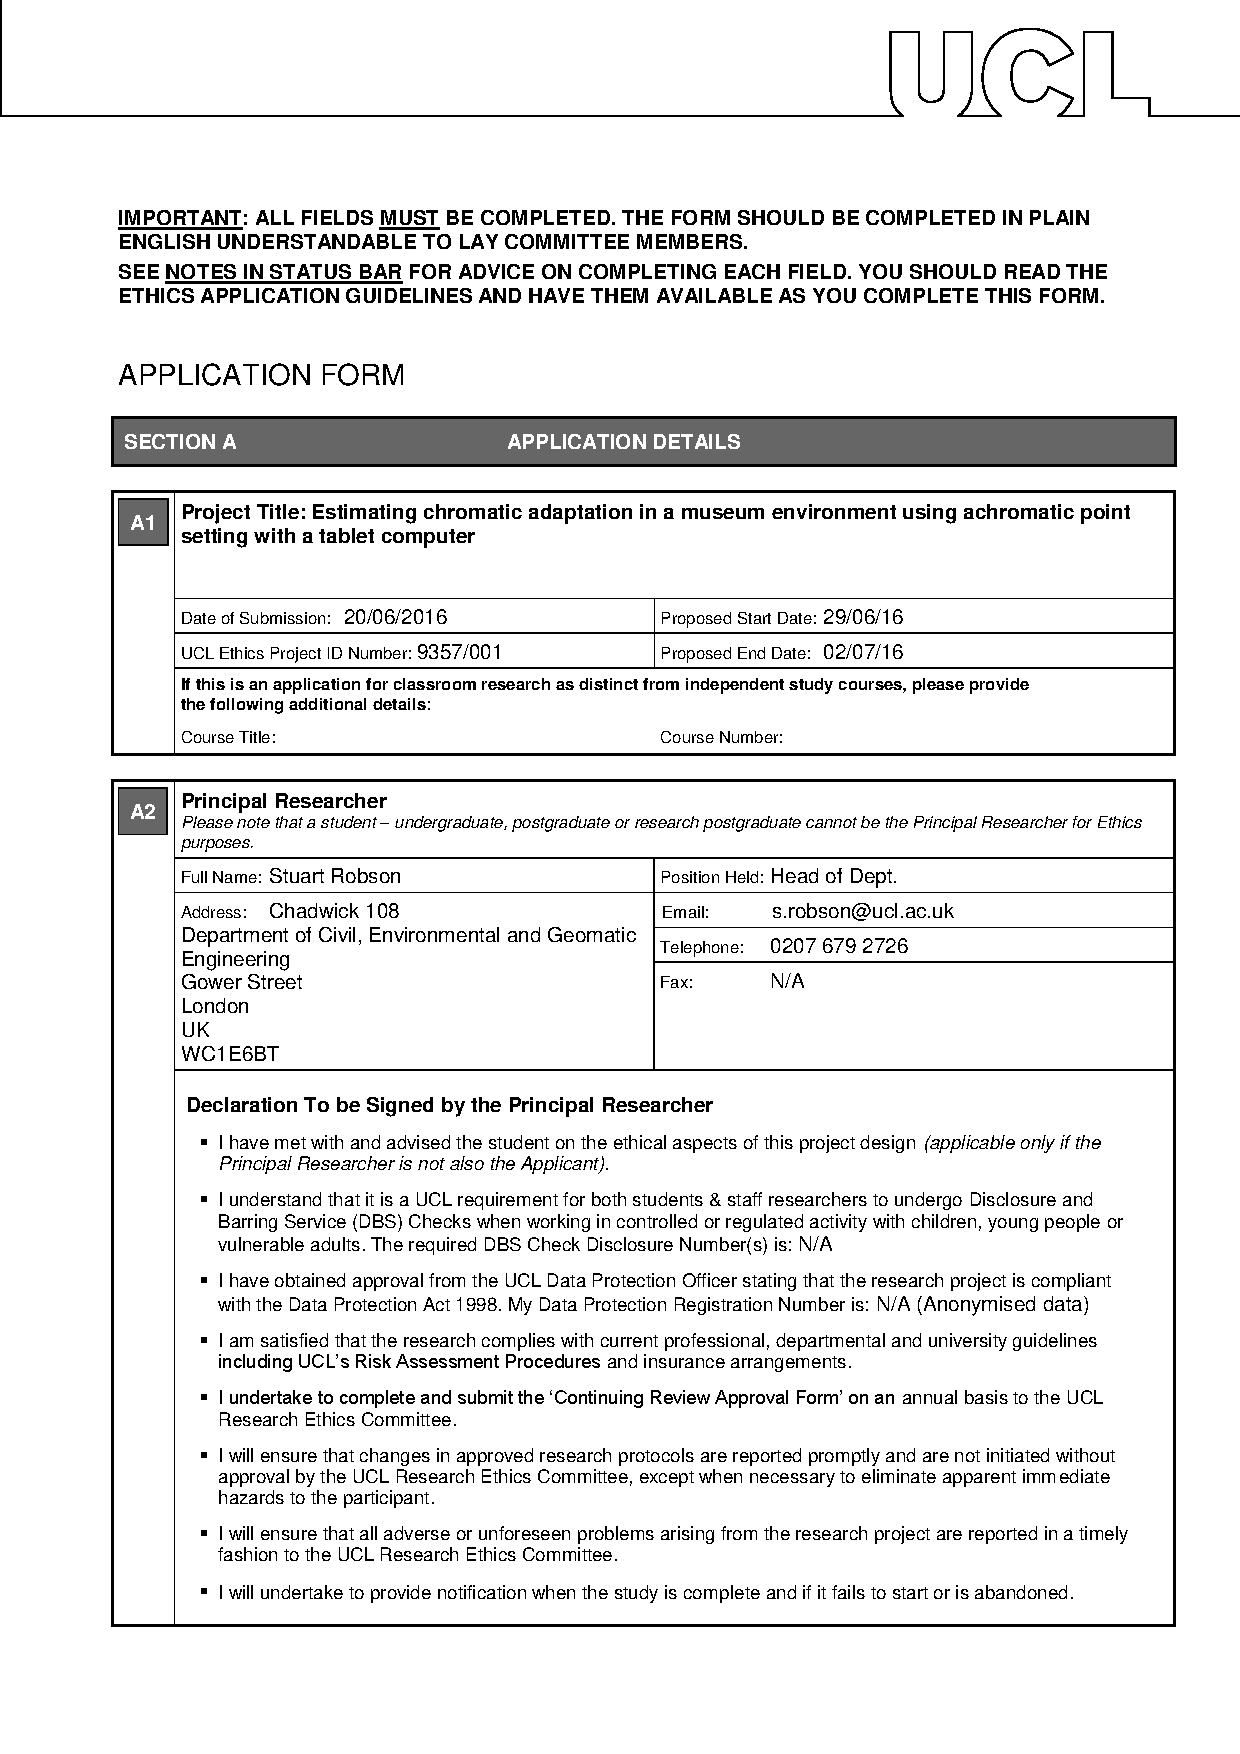
\includepdf[pages=-,scale=0.8]{ethics.pdf}
\chapter{Ethics Application 9357/001 - Amendment}
\label{app:ethics2}
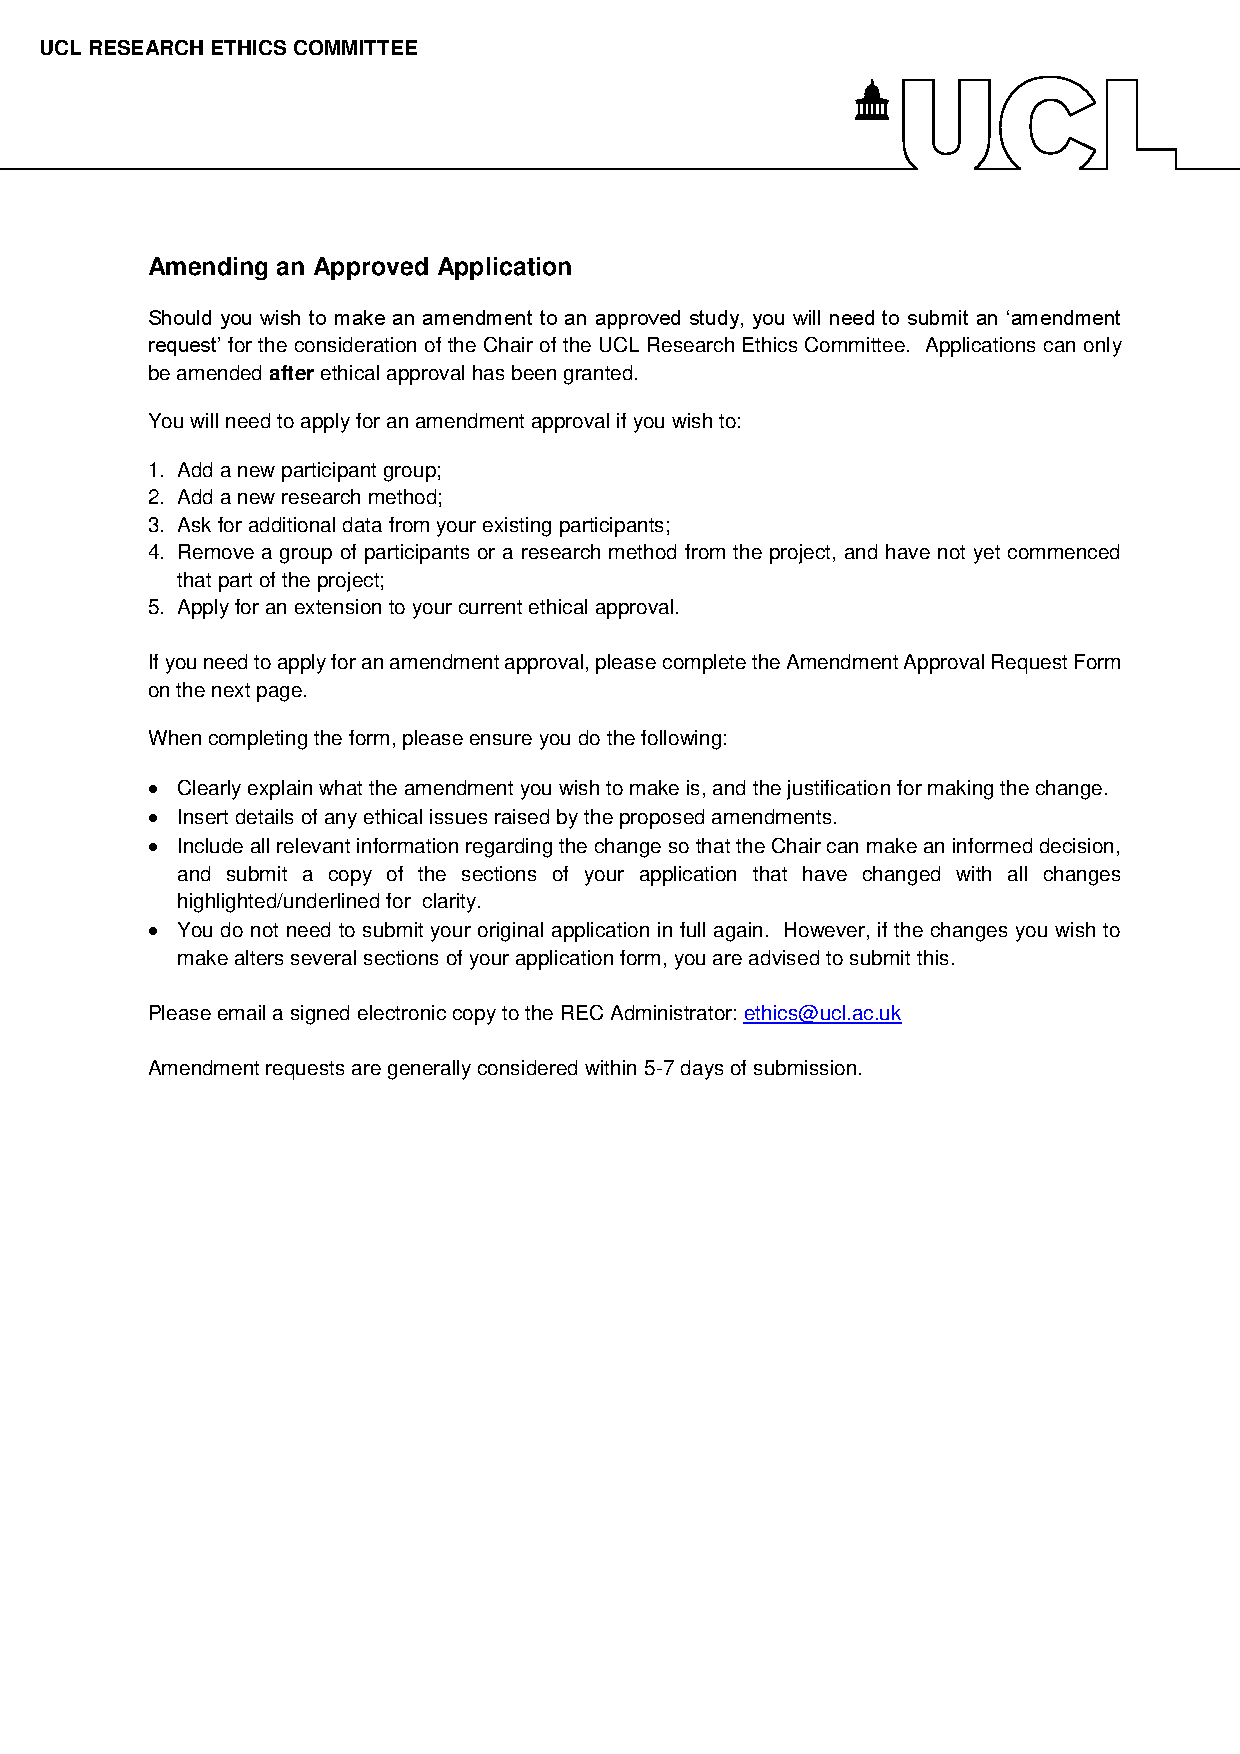
\includepdf[pages=-,scale=0.8]{ethics2.pdf}

